% Standalone, paper-quality TikZ source for the SpECTRE XCTS initial-data
% dependency DAGs (z4c-CCM mission). Compile with:  pdflatex xcts_dag.tex
%
% Style matches the Z4c-CCM derivation-chain figure in
% paper/z4c-CMM/zccm_formulation/sections/matching.tex:
%   - black "box" nodes   : shared / foundational components (identical code)
%   - dark-blue "newbox"  : new / swapped (problem-specific) content
%   - gray Latex-tipped "arr" arrows.
\documentclass[tikz,border=6pt]{standalone}
\usepackage{amsmath}
\usepackage{amssymb}
\usepackage[T1]{fontenc}
\usepackage[dvipsnames,usenames]{xcolor}
\usetikzlibrary{positioning,arrows.meta,fit,backgrounds,calc}

\begin{document}

%======================================================================
% DAG 1: BBH vs Teukolsky XCTS -- shared spine, branched leaves.
%======================================================================
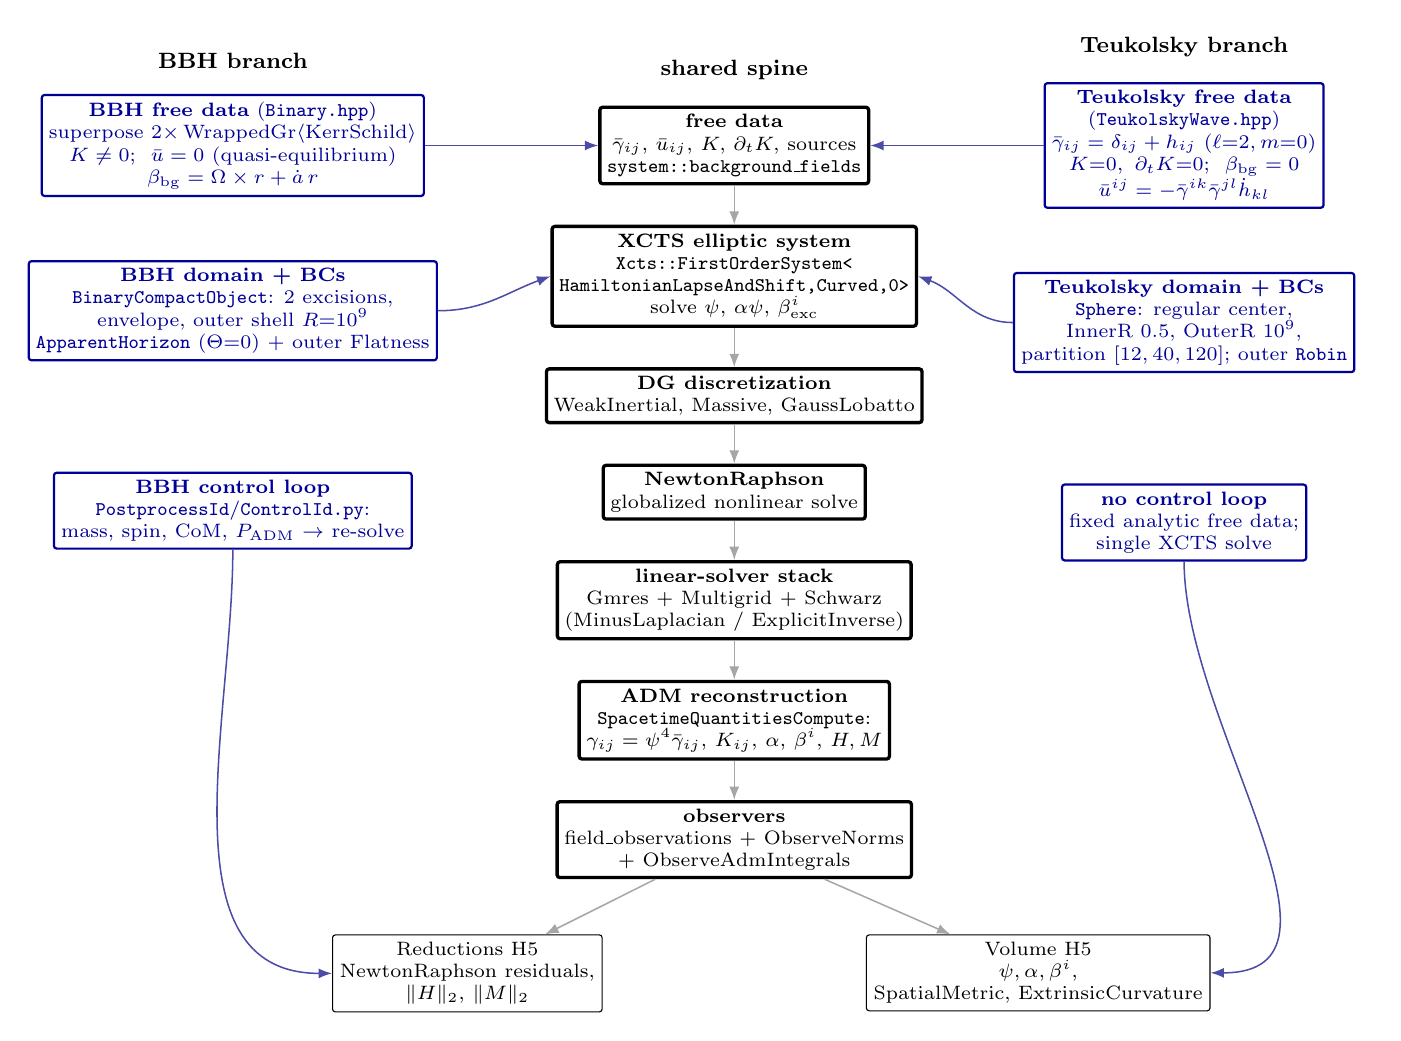
\begin{tikzpicture}[
  node distance = 5mm and 9mm,
  box/.style    = {draw, rounded corners=1pt, align=center,
                   font=\scriptsize, inner sep=2.6pt, fill=white},
  share/.style  = {box, draw=black, very thick},
  newbox/.style = {box, draw=blue!60!black, text=blue!60!black, thick},
  arr/.style    = {-{Latex[length=1.7mm]}, line width=0.55pt, gray!70},
  arrb/.style   = {-{Latex[length=1.7mm]}, line width=0.55pt, blue!50!black!70},
]

% ---- central shared spine (top -> bottom) ----
\node[share] (free)   {\textbf{free data}\\ $\bar\gamma_{ij},\,\bar u_{ij},\,K,\,\partial_t K,$ sources\\ \texttt{system::background\_fields}};
\node[share, below=of free] (sys)  {\textbf{XCTS elliptic system}\\ \texttt{Xcts::FirstOrderSystem<}\\ \texttt{HamiltonianLapseAndShift,Curved,0>}\\ solve $\psi,\,\alpha\psi,\,\beta^i_{\rm exc}$};
\node[share, below=of sys] (dg)    {\textbf{DG discretization}\\ WeakInertial, Massive, GaussLobatto};
\node[share, below=of dg] (nr)     {\textbf{NewtonRaphson}\\ globalized nonlinear solve};
\node[share, below=of nr] (ls)     {\textbf{linear-solver stack}\\ Gmres $+$ Multigrid $+$ Schwarz\\ (MinusLaplacian / ExplicitInverse)};
\node[share, below=of ls] (adm)    {\textbf{ADM reconstruction}\\ \texttt{SpacetimeQuantitiesCompute}:\\ $\gamma_{ij}=\psi^4\bar\gamma_{ij},\,K_{ij},\,\alpha,\,\beta^i,\,H,M$};
\node[share, below=of adm] (obs)   {\textbf{observers}\\ field\_observations $+$ ObserveNorms\\ $+$ ObserveAdmIntegrals};

% ---- output fan-out ----
\node[box, below left=7mm and -6mm of obs] (red) {Reductions H5\\ NewtonRaphson residuals,\\ $\|H\|_2,\,\|M\|_2$};
\node[box, below right=7mm and -6mm of obs] (vol) {Volume H5\\ $\psi,\alpha,\beta^i,$\\ SpatialMetric, ExtrinsicCurvature};

% ---- BBH branch (left) ----
\node[newbox, left=22mm of free] (bbhfd) {\textbf{BBH free data} (\texttt{Binary.hpp})\\ superpose $2\times$\,WrappedGr$\langle$KerrSchild$\rangle$\\ $K\neq0$;\ \ $\bar u=0$ (quasi-equilibrium)\\ $\beta_{\rm bg}=\Omega\times r+\dot a\,r$};
\node[newbox, below=8mm of bbhfd] (bbhdom) {\textbf{BBH domain + BCs}\\ \texttt{BinaryCompactObject}: 2 excisions,\\ envelope, outer shell $R{=}10^9$\\ \texttt{ApparentHorizon} ($\Theta{=}0$) $+$ outer Flatness};
\node[newbox, below=14mm of bbhdom] (bbhctl) {\textbf{BBH control loop}\\ \texttt{PostprocessId}/\texttt{ControlId.py}:\\ mass, spin, CoM, $P_{\rm ADM}$ $\to$ re-solve};

% ---- Teukolsky branch (right) ----
\node[newbox, right=22mm of free] (tkfd) {\textbf{Teukolsky free data}\\ (\texttt{TeukolskyWave.hpp})\\ $\bar\gamma_{ij}=\delta_{ij}+h_{ij}$ ($\ell{=}2,m{=}0$)\\ $K{=}0,\ \partial_t K{=}0$;\ \ $\beta_{\rm bg}=0$\\ $\bar u^{ij}=-\bar\gamma^{ik}\bar\gamma^{jl}\dot h_{kl}$};
\node[newbox, below=8mm of tkfd] (tkdom) {\textbf{Teukolsky domain + BCs}\\ \texttt{Sphere}: regular center,\\ InnerR $0.5$, OuterR $10^9$,\\ partition $[12,40,120]$;\ outer \texttt{Robin}};
\node[newbox, below=14mm of tkdom] (tkctl) {\textbf{no control loop}\\ fixed analytic free data;\\ single XCTS solve};

% ---- edges: spine ----
\draw[arr] (free) -- (sys);
\draw[arr] (sys)  -- (dg);
\draw[arr] (dg)   -- (nr);
\draw[arr] (nr)   -- (ls);
\draw[arr] (ls)   -- (adm);
\draw[arr] (adm)  -- (obs);
\draw[arr] (obs)  -- (red);
\draw[arr] (obs)  -- (vol);

% ---- edges: branches into the spine ----
\draw[arrb] (bbhfd.east) -- (free.west);
\draw[arrb] (tkfd.west)  -- (free.east);
\draw[arrb] (bbhdom.east) to[out=0,in=200] (sys.west);
\draw[arrb] (tkdom.west)  to[out=180,in=340] (sys.east);
\draw[arrb] (bbhctl.south) to[out=270,in=180] (red.west);
\draw[arrb] (tkctl.south)  to[out=270,in=0]   (vol.east);

% ---- column headers ----
\node[font=\footnotesize\bfseries, above=2mm of bbhfd] {BBH branch};
\node[font=\footnotesize\bfseries, above=2mm of free]  {shared spine};
\node[font=\footnotesize\bfseries, above=2mm of tkfd]  {Teukolsky branch};

\end{tikzpicture}

\bigskip\bigskip

%======================================================================
% DAG 2: XCTS generation usage graph (author -> consume).
%======================================================================
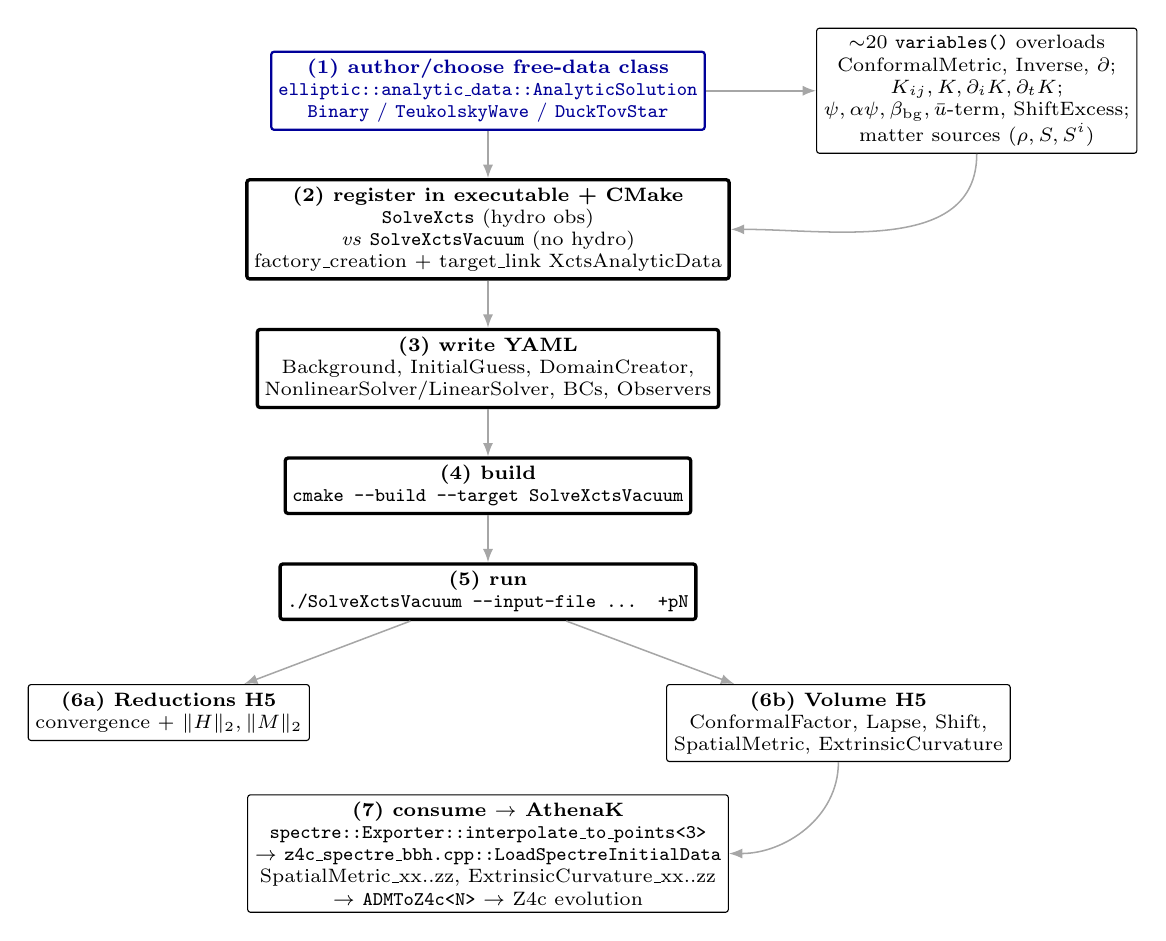
\begin{tikzpicture}[
  node distance = 6mm and 10mm,
  box/.style    = {draw, rounded corners=1pt, align=center,
                   font=\scriptsize, inner sep=2.6pt, fill=white},
  stepbox/.style   = {box, draw=black, very thick},
  newbox/.style = {box, draw=blue!60!black, text=blue!60!black, thick},
  arr/.style    = {-{Latex[length=1.7mm]}, line width=0.55pt, gray!70},
]

\node[newbox] (author) {\textbf{(1) author/choose free-data class}\\ \texttt{elliptic::analytic\_data::AnalyticSolution}\\ \texttt{Binary} / \texttt{TeukolskyWave} / \texttt{DuckTovStar}};
\node[box, right=14mm of author] (vars) {$\sim$20 \texttt{variables()} overloads\\ ConformalMetric, Inverse, $\partial$;\\ $K_{ij},K,\partial_iK,\partial_tK$;\\ $\psi,\alpha\psi,\beta_{\rm bg},\bar u$-term, ShiftExcess;\\ matter sources $(\rho,S,S^i)$};
\node[stepbox, below=of author] (reg) {\textbf{(2) register in executable + CMake}\\ \texttt{SolveXcts} (hydro obs)\\ \emph{vs} \texttt{SolveXctsVacuum} (no hydro)\\ factory\_creation + target\_link XctsAnalyticData};
\node[stepbox, below=of reg] (yaml) {\textbf{(3) write YAML}\\ Background, InitialGuess, DomainCreator,\\ NonlinearSolver/LinearSolver, BCs, Observers};
\node[stepbox, below=of yaml] (build) {\textbf{(4) build}\\ \texttt{cmake --build --target SolveXctsVacuum}};
\node[stepbox, below=of build] (run) {\textbf{(5) run}\\ \texttt{./SolveXctsVacuum --input-file ... +pN}};

\node[box, below left=8mm and -4mm of run] (red2) {\textbf{(6a) Reductions H5}\\ convergence $+$ $\|H\|_2,\|M\|_2$};
\node[box, below right=8mm and -4mm of run] (vol2) {\textbf{(6b) Volume H5}\\ ConformalFactor, Lapse, Shift,\\ SpatialMetric, ExtrinsicCurvature};

\node[box, below=22mm of run] (consume) {\textbf{(7) consume $\to$ AthenaK}\\ \texttt{spectre::Exporter::interpolate\_to\_points<3>}\\ $\to$ \texttt{z4c\_spectre\_bbh.cpp::LoadSpectreInitialData}\\ SpatialMetric\_xx..zz, ExtrinsicCurvature\_xx..zz\\ $\to$ \texttt{ADMToZ4c<N>} $\to$ Z4c evolution};

\draw[arr] (author) -- (vars);
\draw[arr] (vars.south) to[out=270,in=0] (reg.east);
\draw[arr] (author) -- (reg);
\draw[arr] (reg) -- (yaml);
\draw[arr] (yaml) -- (build);
\draw[arr] (build) -- (run);
\draw[arr] (run) -- (red2);
\draw[arr] (run) -- (vol2);
\draw[arr] (vol2.south) to[out=270,in=0] (consume.east);

\end{tikzpicture}

\end{document}
